
\section{SIMULADOR E TESTES}

O desenvolvimento e os testes utilizaram o simulador no
time da UNESP-Bauru previamente existente. O simulador
executa o m{\'o}dulo de estrat{\'e}gia e o de controle, oriundos do
software executado para o ambiente real, sem altera{\c c}ões nos
c{\'o}digos. Apenas os arquivos de c{\'o}digos dos dois m{\'o}dulos
(estrat{\'e}gia e controle) da pasta de fontes destinado ao ambiente
real precisam ser transportados para a pasta do simulador,
nenhuma outra altera{\c c}{\~a}o precisa ser realizada. Apesar da
din{\^a}mica ser pouco considerada neste simulador, ele simplifica
a realiza{\c c}{\~a}o de testes dos algoritmos em desenvolvimento, sem
a necessidade da montagem do ambiente real. Uma imagem do
simulador em uma situa{\c c}{\~a}o de jogo pode ser na vista na Fig. 5.
O simulador pode tamb{\'e}m apresentar o campo potencial
gerado pelo m{\'o}dulo de controle, Fig. 6.

% FIGURA 5
\begin{figure}[!htb]
\centering
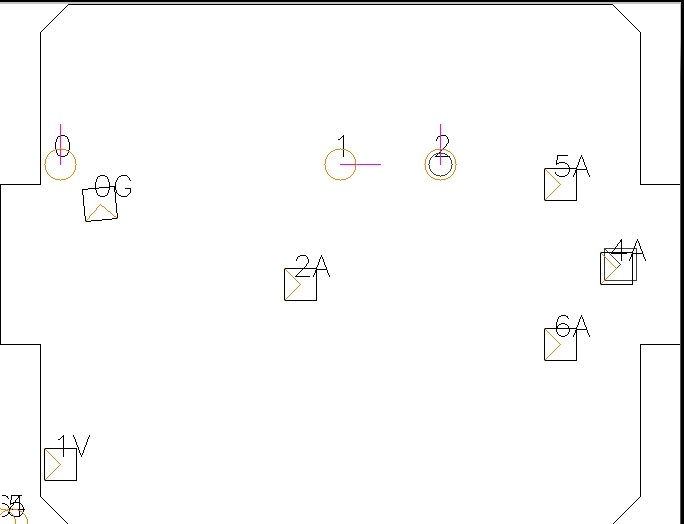
\includegraphics[scale=0.4]{simulador.png}
\caption{Situa{\c c}{\~a}o representada pelo simulador.}
\label{Rotulo}
\end{figure}
%%%

% FIGURA 6
\begin{figure}[!htb]
\centering
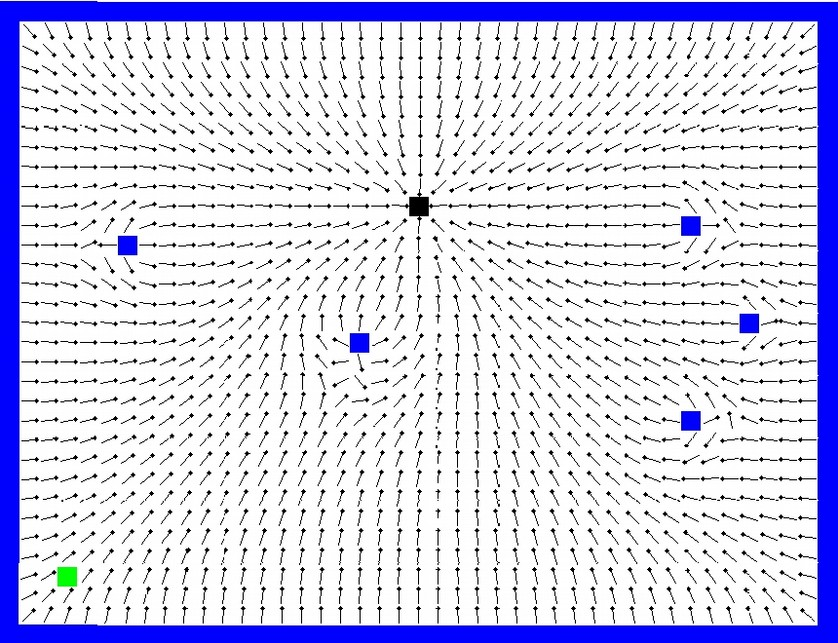
\includegraphics[scale=0.3]{simulador_CP.png}
\caption{Representa{\c c}{\~a}o do campo potencial para a situa{\c c}{\~a}o apresentada na
Fig. 5 considerando o rob{\^o} 1V (volante). Nos quais os quadrados preto, verde
e azul representam respectivamente meta, rob{\^o} e obst{\'a}culo.}
\label{Rotulo}
\end{figure}
%%%

Para que os teste pudessem gerar an{\'a}lises convincentes em
rela{\c c}{\~a}o ao desenvolvimento da estrat{\'e}gia e do controle, foi
necess{\'a}rio acrescentar uma nova funcionalidade que
permitisse dois times jogarem entre si. Para isso foi
desenvolvido no c{\'o}digo do simulador a possibilidade de se
comunicar em rede, de tal forma que houvessem dois times
clientes, cada um com sua estrat{\'e}gia e controle, se
comunicando com o servidor do simulador, que efetiva os
comandos enviados por cada cliente, realizando a
movimenta{\c c}{\~a}o dos rob{\^o}s e da bola virtualmente, e fazendo o
papel da vis{\~a}o ao fornecer o estado de cada rob{\^o} para os times
clientes. Para a comunica{\c c}{\~a}o entre os clientes e o servidor
optou-se por um protocolo de comunica{\c c}{\~a}o simples, o User
Datagram Protocol (UDP).

Desta forma mudou-se a forma como o simulador funciona.
Na Fig. 7 {\'e} apresentado o esquema, de forma simplificada, do
simulador antigo, em que a estrat{\'e}gia recebe o estado do rob{\^o},
calcula o objetivo e envia para o controle. O controle vai
calcular a trajet{\'o}ria e o comando que ser{\'a} enviado para cada
roda, que ser{\'a} enviado para o simulador que efetua a
movimenta{\c c}{\~a}o.

% FIGURA 7
\begin{figure}[!htb]
\centering
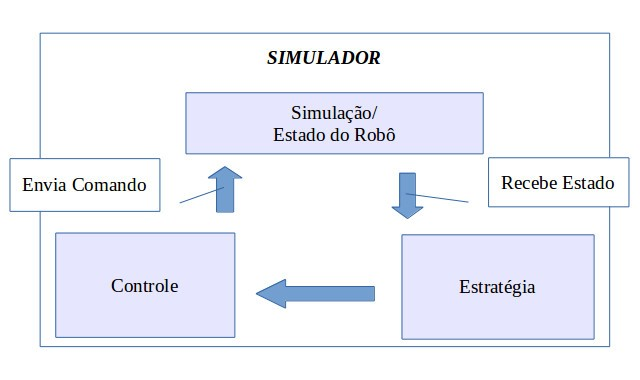
\includegraphics[scale=0.5]{esquema_simulador.png}
\caption{Simulador antes das altera{\c c}{\~o}es.}
\label{Rotulo}
\end{figure}
%%%

Na Fig. 8 {\'e} apresentado o esquema do simulador atual, no
qual o simulador torna-se um servidor, que recebe os
comandos de cada roda, efetua-os e em seguida envia o estado
do rob{\^o} para os clientes. Os clientes recebem o estado,
calculam o objetivo atrav{\'e}s da estrat{\'e}gia e os comandos a ser
enviados para o simulador atrav{\'e}s do controle, na sequ{\^e}ncia
esse comando {\'e} enviado para o servidor que efetuar{\'a} a
movimenta{\c c}{\~a}o dos rob{\^o}s. Al{\'e}m disso, tem-se a representa{\c c}{\~a}o
para a conex{\~a}o de um cliente, mas a representa{\c c}{\~a}o {\'e} a mesma
para dois clientes, que {\'e} o caso do futebol de rob{\^o}s.

% FIGURA 8
\begin{figure}[!htb]
\centering
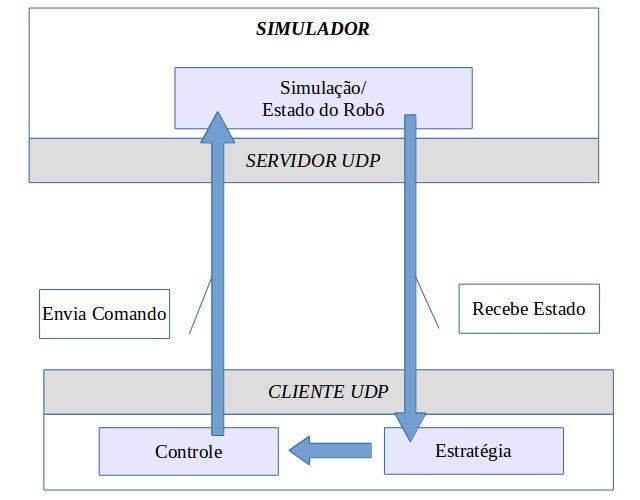
\includegraphics[scale=0.5]{esqumatica_simulador.png}
\caption{ Simulador ap{\'o}s altera{\c c}{\~o}es, representando uma conex{\~a}o.}
\label{Rotulo}
\end{figure}
%%%

Assim, o novo simulador permite intera{\c c}{\~a}o entre dois times
virtuais, levando em considera{\c c}{\~a}o a din{\^a}mica, cinem{\'a}tica e
demais constantes f{\'i}sicas referentes ao rob{\^o} do time Carrossel
Caipira, possibilitando a compara{\c c}{\~a}o atrav{\'e}s de estat{\'i}sticas
que podem ser coletadas durante a execu{\c c}{\~a}o do programa, na
figura 9 temos a imagem do novo simulador.

% FIGURA 9
\begin{figure}[!htb]
\centering
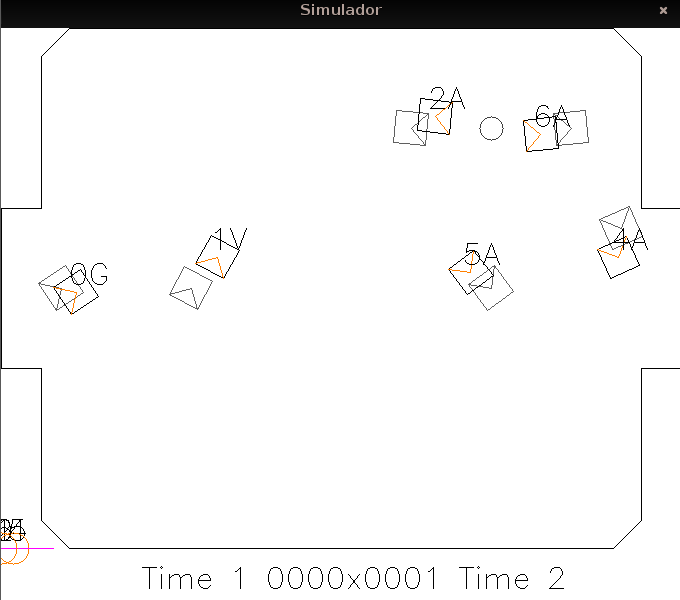
\includegraphics[scale=0.48]{simulador2.png}
\caption{ Simulador ap{\'o}s altera{\c c}{\~o}es, representando uma conex{\~a}o.}
\label{Rotulo}
\end{figure}
%%%

Nesta vers{\~a}o, o simulador procura entender o
comportamento da estrat{\'e}gia e controle estudados, atrav{\'e}s de
situa{\c c}ões de jogo como: placar total, gols contra, p{\^e}naltis
usufru{\'i}do pelo time Carrossel Caipira para o desenvolvimento
das pesquisas envolvendo futebol de cometidos, p{\^e}naltis
convertidos, gols de cada rob{\^o}, n{\'u}mero de free balls e tempo de
jogo. Al{\'e}m disto, {\'e} poss{\'i}vel verificar a evolu{\c c}{\~a}o do placar no
decorrer da simula{\c c}{\~a}o e avaliar o intervalo de confian{\c c}a para
estimar a margem de erro dos dados levantados. A an{\'a}lise
quantitativa dos dados estimula a an{\'a}lise com dados reais feita
no ambiente controlado do laborat{\'o}rio que complementa o
ambiente instrumental rob{\^o}s. 
